\chapter{模型评价}
\label{cha:evaluation}

我们尝试用 $2^{16}$ 个真实的 IPv6 地址训练贝叶斯网络模型, 然后利用该模型生成 256 个候选 IPv6 地址进行扫描, 并对扫描结果进行评估.

图~\ref{fig:generate}~显示了部分生成的 IPv6 地址. 图~\ref{fig:scan}~显示了使用 nmap 程序扫描生成的地址的结果.

\begin{figure}[htbp]
\centering
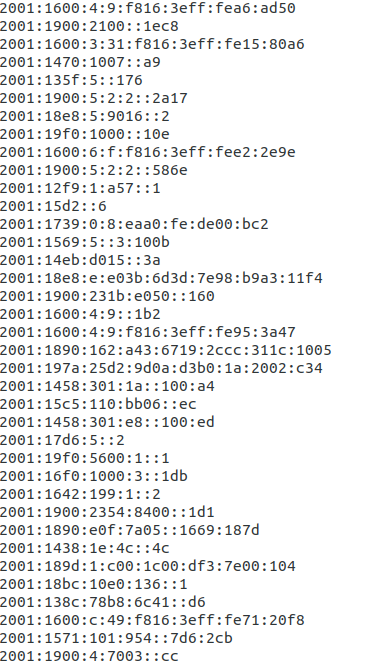
\includegraphics[width=0.3\textwidth]{generate}
\caption{地址生成}
\label{fig:generate}
\end{figure}

\begin{figure}[htbp]
\centering
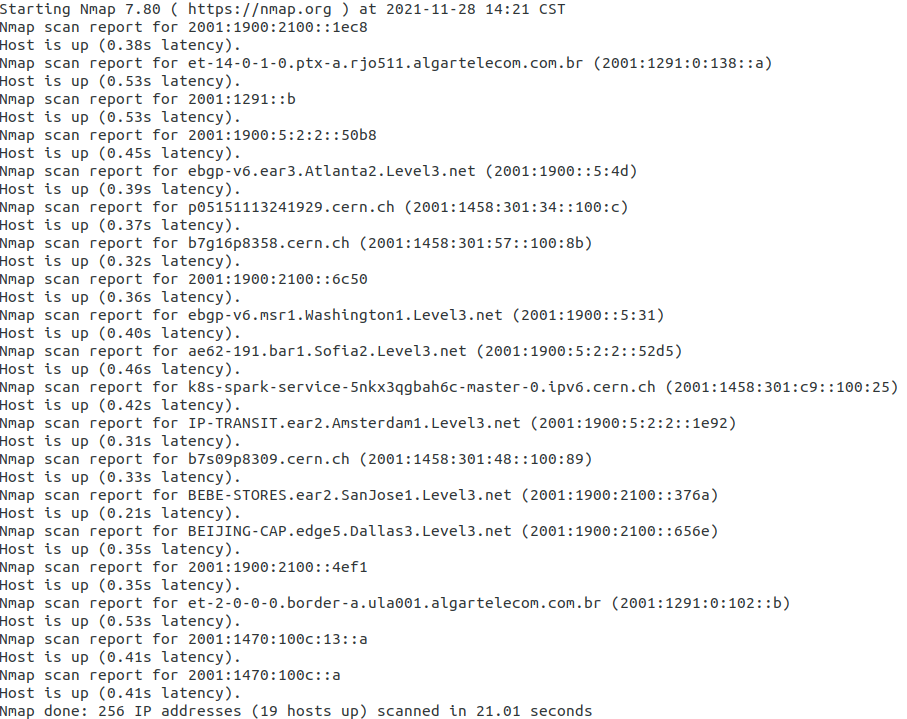
\includegraphics[width=0.5\textwidth]{scan}
\caption{地址扫描}
\label{fig:scan}
\end{figure}

生成的地址中约 7\% 是存活的, 该结果表明本文提出的基于贝叶斯网络的 IPv6 地址生成模型是一个卓有成效的 IPv6 网络扫描方法.
